% !TEX root = ../main.tex
%
\chapter{Conclusions} \label{sec:5}

The aim of this thesis work was to explore the possibility to observe the \dst dibaryon in \pPb collisions 
at \sctev with the ALICE experiment.
The importance of this search lies in the fact that the measurement of the \ds signal would be the first
confirmation of the existence of non-trivial dibaryons.

The identification of the \ds is challenging because of the experimental condition of the 
\pPb collisions. The choice of the \pPb data sample for this study was dictated by the necessity to have 
the maximum number of deuterons.
In fact the 2016 \pPb data sample is the ALICE sample with the greatest number of deuterons, excluding \PbPb
data. 
The \PbPb data was not considered because of the high particle multiplicity produced in this colliding
system that generates a huge combinatorial background that makes the \ds identification very difficult.
In pp collisions, instead, the deuteron production is lower than in \pPb by a factor $\sim 3$, therefore
was a priori excluded.

Nevertheless, the study of the background in \pPb collisions, performed in this thesis, showed that the
combinatorial background due to pions is crucial also in this colliding system and prevent the clear 
identification of the \ds decay. 
The wide shape of the \ds resonance, also contribute to make its identification even harder.
This results in a low significance, < 0.25, for the measurement of the \ds signal \ -- assuming that \ds
is produced according to the Thermal model.

Upper limits was set for the production of the \ds dibaryon in \pPb collisions at \sctev, since there is
no evidence of its presence in the analysed data sample. The low significance of the measurement, however, 
leads to weak limits, thus it is not possible to exclude that \ds is produced according to the Thermal
model.

The detailed studies performed for this thesis work have given a clearer picture of the 
problems related to the search of the \ds dibaryon with the ALICE experiment. 
Furthermore, the analysis tools and methods developed for this work can be used in future analysis.
Now it is clear that significant results can be achieved only increasing the significance of the
measurement.
The low significance of the measurement can be improved, basically, in two ways: reducing the 
combinatorial background and increasing the integrated luminosity.

A significant background reduction could be obtained searching the \ds in pp collisions.
alla luce dei risultati di questa tesi la minor
minore abbondanza di deutoni in questo sistema di collisione potrebbe essere 
essere compensata dalla riduzione dalla riduzione del fondo combinatoriale dovuto ai pioni 
(il numero di combinatori scala come una potenza del numero dei pioni).
Inoltre in pp è possibile fare PID con l'ITS standalone migliorando l'efficienza.

The search of the \ds in pp collisions was initially (scartata) excluded due to the minor deuteron 
production, bu this thesis shown that can be more convenient to look in pp data. 

\begin{figure} [htb]
    \centering
    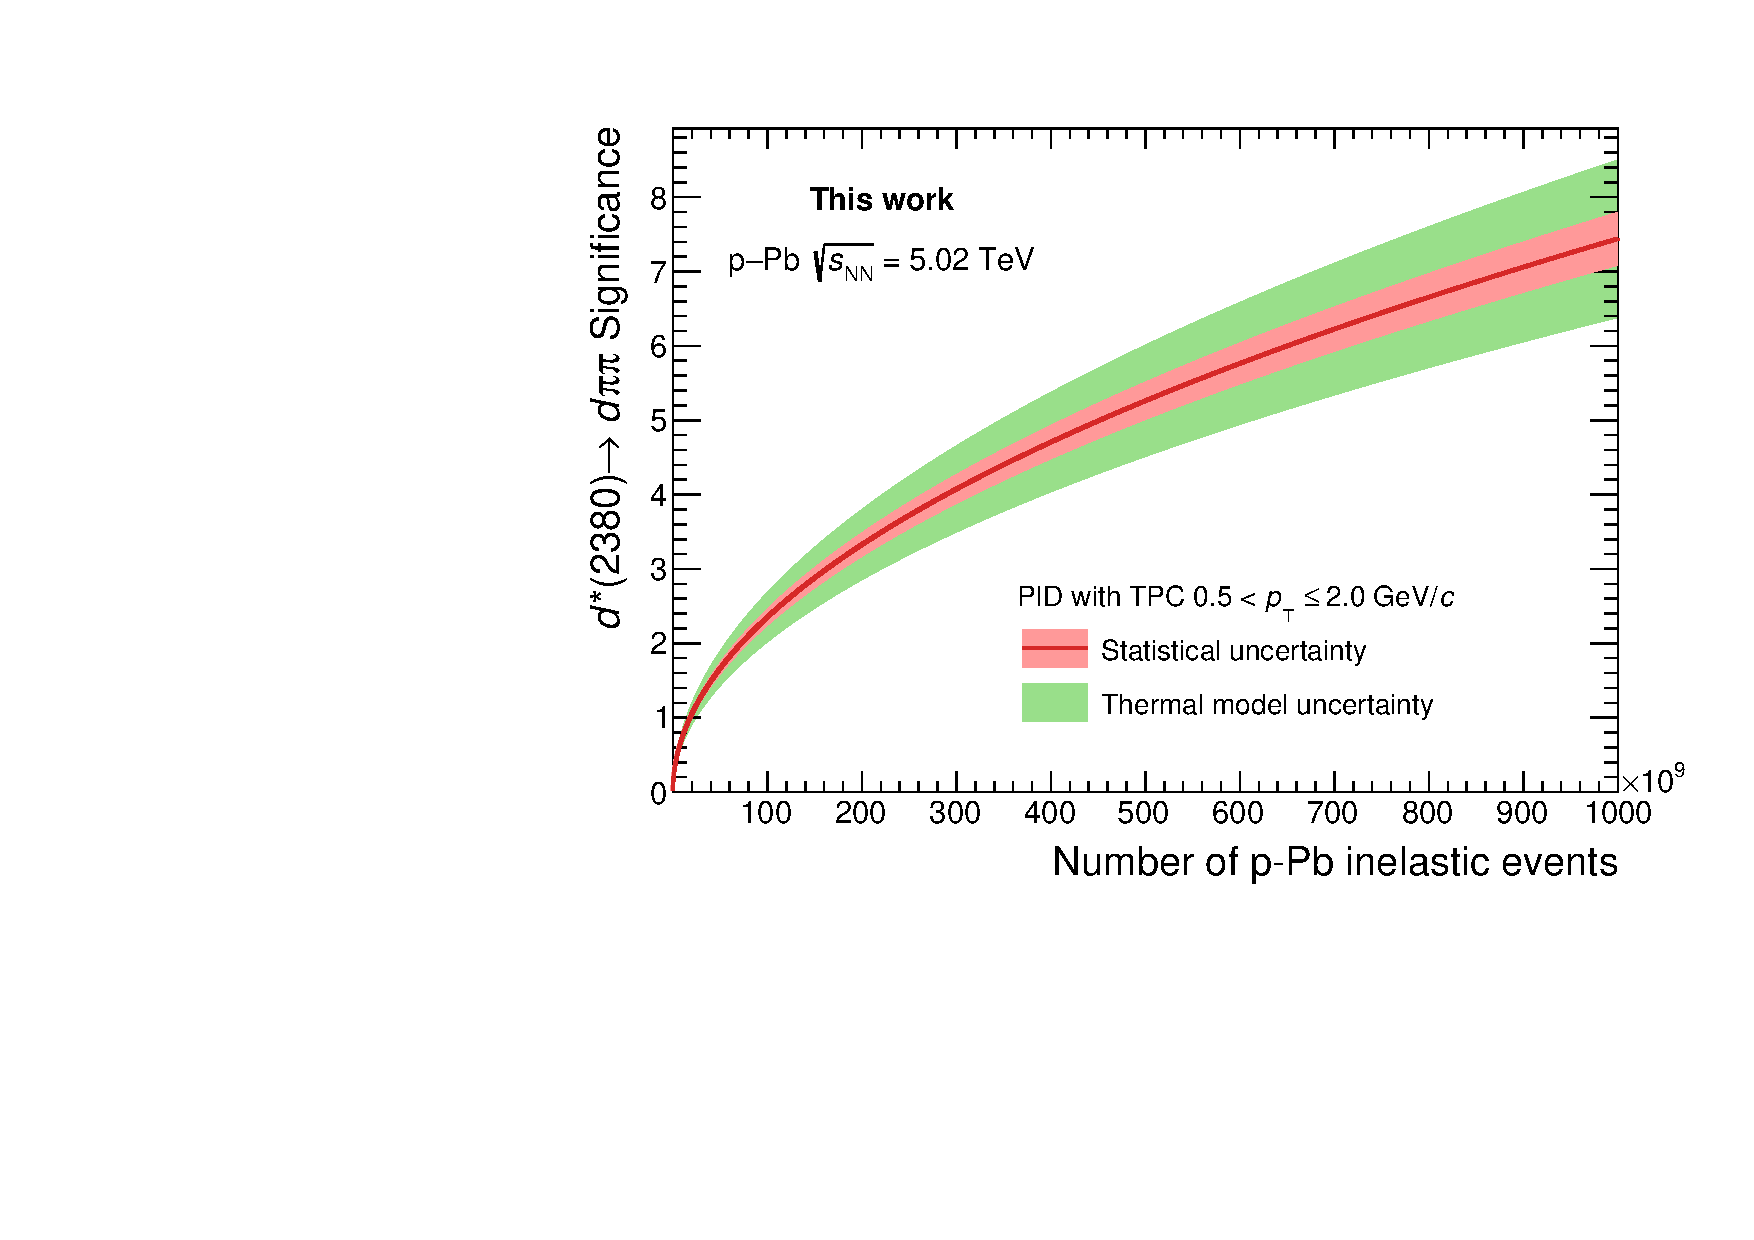
\includegraphics[width=0.85\textwidth]{gfx/sig_TPC}
    \caption{Upper limit on the double-differential \ds yield as a function of the \pt. The blue (dashed) lines indicate the expectation of the thermal model assuming a temperature of 156 MeV.}
	\label{fig:proj1}
\end{figure}

A final study was performed in order to estimate the number of \pPb collisions needed to reach 
$5\;\sigma$ significance.
Figure~\ref{fig:proj1} show that $\sim 5\times10^{11}$ events are needed tho achieve this goal with the
TPC configuration.
This number if far greater than the number of \pPb collisions available in the 2016 data sample
\ -- $5.5\times10^{8}$ minimum bias events.
This integrated luminosity is planned to be reached during the LHC Run 3 which will start in 2021.
Therefore the search of the \ds dibaryon with the ALICE experiment will lead to significant results
in the next years, and the experience gained with this work will be crucial.




% Furthermore, in the lights of this work the \ds will be searched also in the pp data using
% the methods developed for this thesis. In pp collisions the pion production is smaller than in \pPb
% and this lead to a smaller combinatorial background. It is also possible to improve the
% particle identification of low momentum particles using the ITS detector,
% increasing the reconstruction efficiency.
% Preliminary studies suggest 


